%\PassOptionsToPackage{demo}{graphicx}
\documentclass[slidestop,compress,11pt,xcolor=dvipsnames]{beamer}
%\documentclass{beamer}
\usepackage[latin1]{inputenc} % remplace utf8 con latin1 si va a compilar en un sistema Windows
\usepackage{times}
\usepackage{mdframed}
\usepackage[T1]{fontenc}
\usepackage[spanish]{babel}
\usepackage[sort]{natbib}
\usepackage{textpos}
%\usepackage{graphicx} %sirve para insertar graficos en varios formatos%
\usepackage{graphicx}
%\usepackage{subcaption}
\usepackage{mathtools}
\usepackage[bars]{beamerthemetree} % Beamer theme v 2.2
\usepackage{multicol}
\usepackage{lmodern}
\usepackage{lipsum}
\usepackage{marvosym}
\usefonttheme{professionalfonts} % font de Latex
%\DeclareGraphicsRule{.png}{png}{.png.bb}{} %al parecer sirve para adaptar el tama�o de los gr�ficos cuando se insertan en Beamer
%\usepackage{beamerthemeshadow} %hay que descargar est� opci�n
\newtheorem{defi}{Definici�n}
\setbeamertemplate{navigation symbols}{}
\setbeamertemplate{caption}[numbered]
\providecommand{\abs}[1]{\lvert#1\rvert}
\providecommand{\norm}[1]{\lVert#1\rVert}

% para Numerar Slides sin modificar el tema
%\newcommand*\oldmacro{}%
%\let\oldmacro\insertshorttitle%
%\renewcommand*\insertshorttitle{%
%\oldmacro\hfill%
%\insertframenumber\,/\,\inserttotalframenumber}

% Agregamos informaci�n del autor y titulo

\title[Econometr�a I (EC402)]
{Econometr�a I (EC402)-II semestre de 2013 \\
Clase \#10 - Introducci�n al uso de Gretl }

\author[Prof. Andr�s M. Casta�o]
{
\includegraphics[height=2cm,width=2.5cm]{ucn.jpg}
\\
% con el del mcr es height=1.5cm,width=4cm
Andr�s M. Casta�o}

\institute[]
{
}

\LARGE
\date[Clase 9]
{Ingenier�a Comercial \\
Universidad Cat�lica del Norte\\

Septiembre 25 de 2013}

%\date{\today}

\useoutertheme{infolines}
\usetheme{Boadilla} %tipo de tema
%\usecolortheme{beaver} %color del tema
\usecolortheme{rose}
\setbeamercovered{dynamic} % dentro de ambientes como itemize o enumerate resalta uno y los demas los pone trasparantes
\useoutertheme{infolines}
\useinnertheme{default} % aspectos dentro del tema (cajas, vi�etas, itemize, enumerate, theorem, footnotes. bibliography. opciones: circles,
% default, rectangles


\begin{document} %inicio del documento

%portada
\begin{frame}
\titlepage
\end{frame}

\section{Qu� es Gretl?}
\begin{frame}
\frametitle{Qu� es Gretl?}
\begin{itemize}
\item <1> Gretl is an acronym for Gnu Regression, Econometrics and Time-series Library. It is a software package for doing econometrics that is easy to use and powerful. It features a very user-friendly interface that makes it snap to use in classroom. Its exibility, extensibility, and accuracy make it well-suited for research as well.
\bigskip
\item <1> Gretl comes with many sample data files and its internet capabilities give you access to several very useful databases served by Wake Forest University.
\end{itemize}
\end{frame}

\section{Installing Gretl}
\begin{frame}
\frametitle{Installing Gretl}
\begin{itemize}
\item <1> To install gretl on your system, you will need to download the appropriate executable file
for the computer platform you are using. For Microsoft Windows users the appropriate site is
http://gretl.sourceforge.net/win32/.
\bigskip
\item <1> Data: http://www.learneconometrics.com/gretl/POE4data.exe.
\end{itemize}

\end{frame}

\section{Gretl Basics}
\begin{frame}
\frametitle{Gretl Basics}
\begin{center}
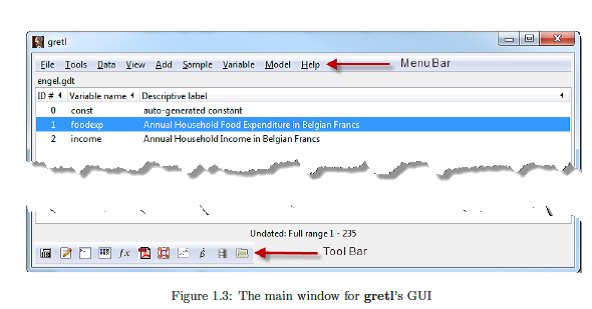
\includegraphics[width=10cm]{grafico1}
\end{center}
\end{frame}

\section{Importing Data}
\begin{frame}
\frametitle{Gretl Basics}
\begin{center}
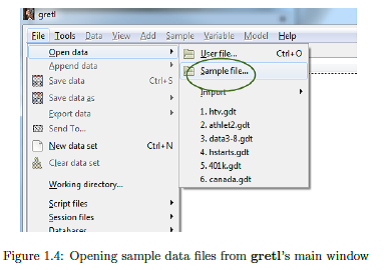
\includegraphics[width=12cm]{grafico2}
\end{center}
\end{frame}

\section{Importing Data}
\begin{frame}
\frametitle{Gretl Basics}
\begin{center}
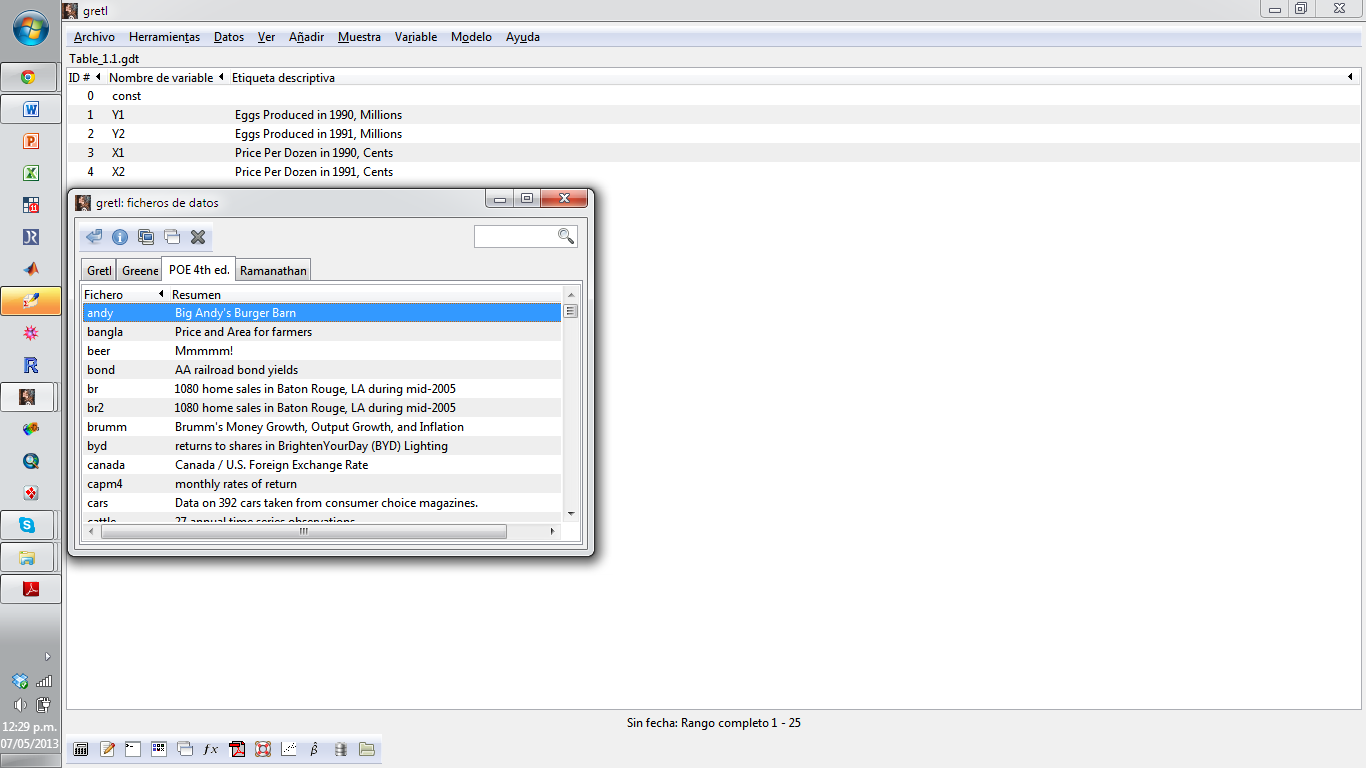
\includegraphics[width=10cm]{grafico3}
\end{center}
\end{frame}

\section{Generating New Variables}
\begin{frame}
\frametitle{Generating New Variables}
\begin{itemize}
\item <1> genr command.
\bigskip
\item <1> Suppose you have a variable in your dataset called food exp. You want to create a new variable as the natural logarithm of food exp. This can be done using series or genr (e.g., series l food exp = ln(food exp).
\end{itemize}
\begin{center}
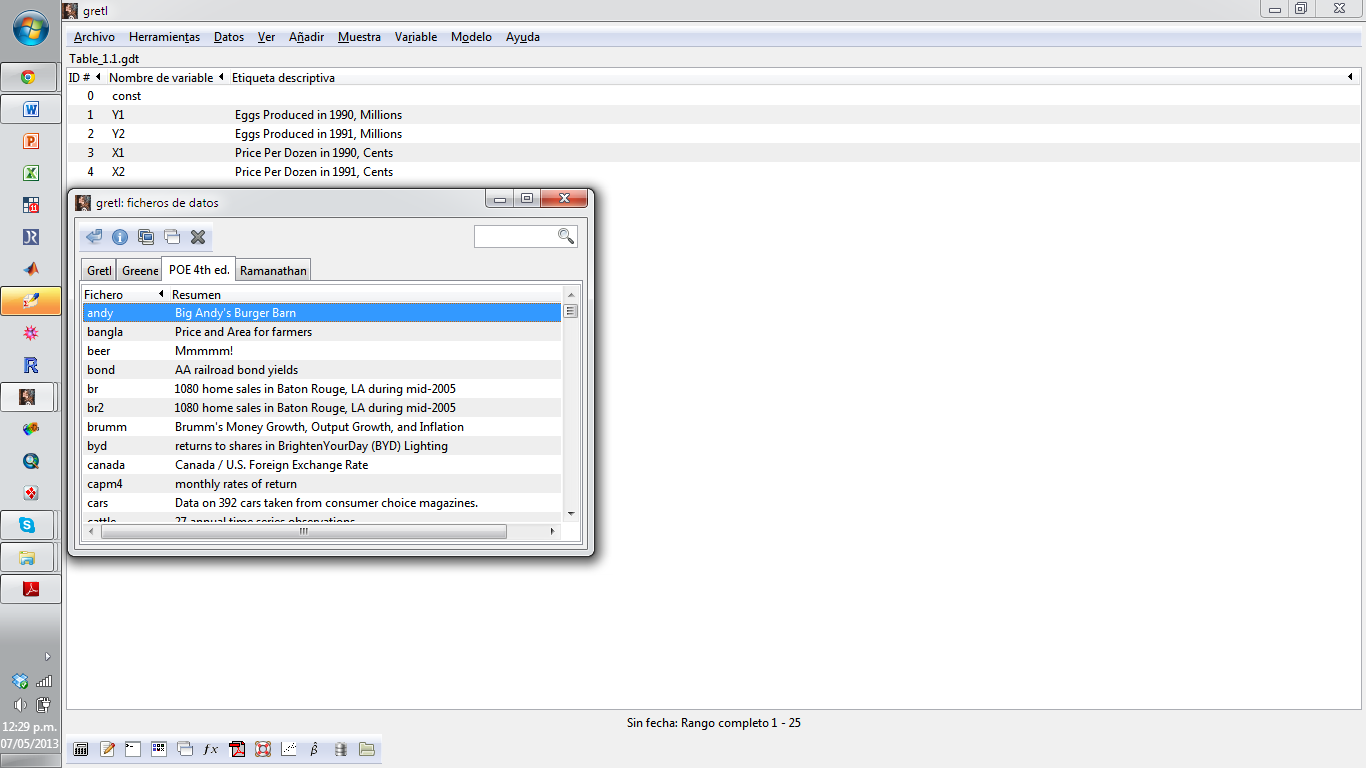
\includegraphics[width=7cm]{grafico3}
\end{center}

\end{frame}


\section{Example: Estimate the Food Expenditure Relationship}
\begin{frame}
\frametitle{Example: Estimate the Food Expenditure Relationship}
The last step is to load the food expenditure and income data into gretl. The data file is included in your gretl sample files-provided that you have installed the Principles of Econometrics data supplement that is available from our website
\begin{center}

\includegraphics[width=10cm]{grafico4}
\end{center}
\end{frame}


\section{Graph the Data}
\begin{frame}
\frametitle{Graph the Data}
\begin{center}
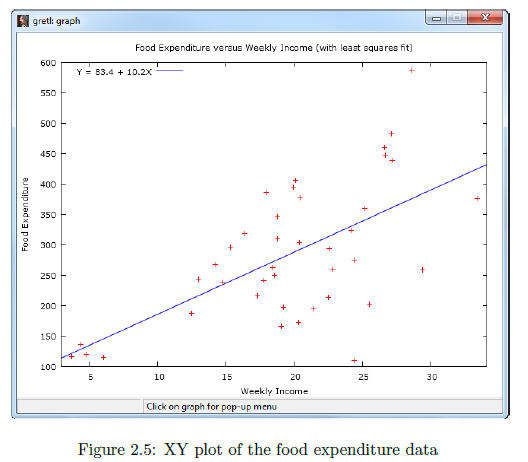
\includegraphics[width=10cm]{grafico5}
\end{center}
\end{frame}


\section{MCO estimation}
\begin{frame}
\frametitle{MCO estimation}
\begin{center}
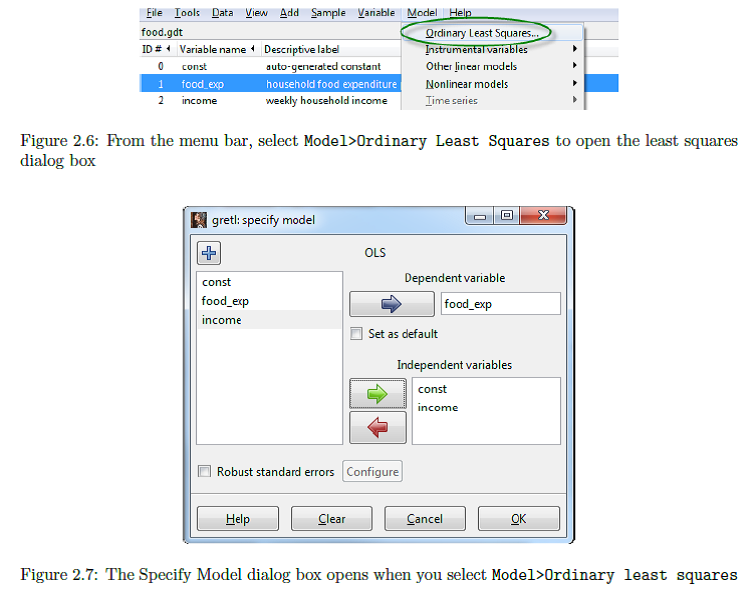
\includegraphics[width=8cm]{grafico6}
\end{center}
\end{frame}


\end{document} 